% 2、内容:包括选题来源、研究意义、国内外研究状况、主要研究内容、拟采取的研究方法、预期研究结果和论文写作计划等。
\chapter{引言}
\section{研究背景与意义}

2023年10月24日,我国政府宣布增发2023年国债1万亿元,集中用于灾后恢复重建和提升国家防灾减灾能力。这一决策表明政府对气候变化带来的灾害风险的高度关注,也突显了防灾减灾工作的紧迫性。在现代社会,气候变化已经成为一个备受瞩目的全球性问题。随着极端气候事件的频繁发生,人们对自身及财产的安全日益关切。在灾害面前,家庭往往是首当其冲的受害者。但与企业相比,个人家庭对这些潜在风险的反应可能更为复杂。家庭是否会通过购买家财险来缓解财产损失,以及他们在灾害发生后是否更加倾向于购买保险,这些问题涉及到家庭的风险认知、保险教育和金融决策等多个方面,具有较强的实证研究价值。

我国的家财险始于1980年,是当时中国人保重点推广的基础险种之一。在1980年,全国范围内有34200户家庭购买了中国人保的家财险,承保金额为5232万元,保费仅为7万元,仅占国内产险保费总额的0.02\%。到了1989年,全国家财险(包括储蓄性两全险)的投保户数增至76,910,000户,承保金额达1974亿元,保费收入为3.2亿元,占产险保费总额的4.4\%。可以说,我国财产保险的早期发展同时也是家庭财产保险演进的历史\citep{黄英君2008论我国产险公司分散性业务营销模式的创新},塑造了国人对财产险最早的认知。然而,随着汽车保有量的急剧增加,财产险公司主要将注意力集中在车险上,导致车险成为财产险中的绝对主导领域,而家财险逐渐被边缘化,稳定增长长期不被关注。

我国家财险近十年保费收入持续提升,市场蓬勃发展但仍与发达国家有所差距。在2013-2021年家财险保费收入从38亿逐步提升至98亿后,2022年家财险以67.22\%的增长率成为了保费增速最快的产险险种,保费达到164亿,但家财险2022年末在行业保费规模中占比仅1.1\%。由于我国城市住宅建筑结构抗风险能力高,对于自然灾害风险暴露较低,因而我国住户对于风险感知度较低,对于保险产品的认知更为有限,保险深度也偏低,存在较大的保障缺口,商业化进展任重而道远。对比国外,美国家财险覆盖率为85\%\citep{croll2018home},2022年市场规模为1483亿美金,约合1.05万亿人民币;日本覆盖率达82\%\citep{plaza},2022年市场规模为1.2万亿日元,约合500亿人民币。可以看出,我国家财险市场仍有较大的发展空间。
% https://mp.weixin.qq.com/s/4PTD5xrrEyDIuoBtbip2sQ
\begin{figure}[H]
    \centering
    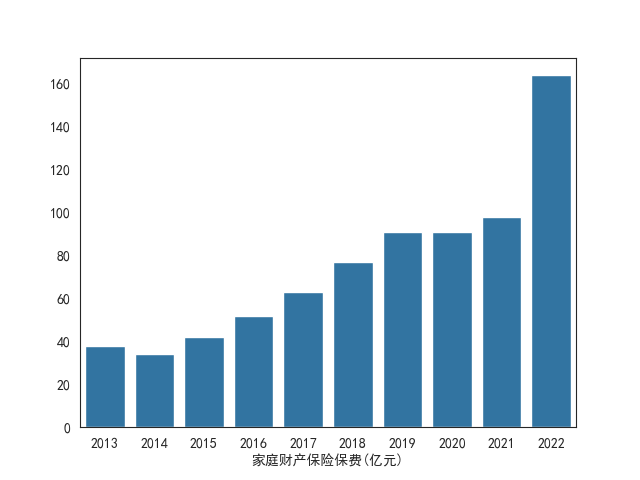
\includegraphics[width=\linewidth]{img/家庭财产保险保费.png}
    \caption{家财险保费持续增长}
\end{figure}

然而,气候变化下人们对自身及财产安全的关切是否能够持续转化为对保险的需求,尤其是在家庭层面,却是一个相对较少被深入研究的领域。过去的国内研究主要关注气候变化对企业财产险或健康险的影响,比如雾霾天导致大量健康险投保之后又退保、位于台风路径上的企业更偏好持有现金\citep{杨娜娜2019自然灾害与企业现金持有}等,但是对于家庭财产保险的定量研究却相对较少。本研究的选题来源于对这一领域的关注,力图深入了解气候变化对家财险需求的影响机制,填补现有研究的空白。

在此背景下,我们将通过深入研究气候变化对家财险需求的影响,探索个人家庭在面对气候变化时的风险管理行为,为保险业和政策制定提供更为全面的了解。本研究的意义不仅仅停留在学术探究层面,更涉及到实际社会和经济层面的多个方面:

首先,通过深入研究气候变化对家财险需求的影响,我们能够为保险公司提供更为精准的市场预测。这对于保险公司的产品开发、定价和风险管理具有重要指导意义。预测气候事件可能引发的家财险需求波动,可以帮助保险公司制定更灵活的营销策略,及时调整产品组合,提高市场适应性。

其次,研究结果还可以为政府和监管机构提供政策制定的依据。随着气候变化对保险市场的影响逐渐显现,相关的监管政策也需要跟进。通过深入了解家庭在面对气候变化时的保险需求变化,政府可以更好地制定相关政策,促进保险市场的健康发展,确保公众的保险保障能力。

此外,研究家财险需求的变化还能够提供社会科学领域对于人类行为和决策的深刻洞察。了解在灾害面前个体的风险认知和行为模式,有助于拓展对人类在危机时刻的心理和社会反应的认知。这对于制定个体和社会层面的应对策略,以及心理健康服务的提供都具有积极的实践意义。

最后,从可持续发展的角度来看,本研究有助于引导人们更加理性和科学地对待气候变化风险。通过了解保险在气候变化应对中的作用,可以提高社会对于个体责任和社会共担责任的认识。这有助于形塑一种更加可持续、共同应对气候挑战的社会文化氛围。

\section{文献综述}

本文主要从两个角度梳理国内外相关文献:一是气候变化对不同保险需求的影响,二是家庭风险偏好的影响因素。

\subsection{气候变化对不同种类保险需求的影响}
关于气候变化对保险需求的影响,有关研究主要集中在寿险、健康险和农险上。其中健康险方面,空气污染水平对健康险的购买或退保的决策产生的显著影响\citep{2018Something},每日空气污染水平每增加一个标准差,当天销售的保险合同数量增加了7.2\%。而在考虑购买后的条件下,即在冷静期内,相对于订单日期水平,每日空气污染水平每减少一个标准差,退保概率增加了4.0\%,研究还探讨了多种可能的机制,发现了对投射偏差和显著性的最有力支持。也有研究旨在探究空气污染对中国居民商业健康保险需求的影响大小\citep{赵强2021空气污染对商业健康保险需求的影响},利用2011年至2016年秦岭淮河地区84个地级市的宏观数据,采用模糊断点回归设计和中国北方集中供暖政策的准自然实验方法,旨在深入了解空气污染对中国居民商业健康保险需求的影响。结果显示,空气污染对商业健康险需求存在显著的正向影响,特别是PM2.5污染物的排放浓度每提升1\%,商业健康保险密度提高1.098\%。即便在考虑六种不同污染物指标的情况下,估计结果仍然趋近一致。值得关注的是,从2013年开始,我国经历了大范围持续的雾霾天气,伴随着新闻媒体报道频率的增加。这导致居民对空气污染的敏感度和重视度逐渐提高,进而反映在对商业健康保险的购买上。

而对于气候变化对健康险需求的影响机制,研究观点主要集中在气候变化影响的个人风险偏好。例如有研究认为空气污染提升了个人的风险感知,进而引起健康保险需求增加\citep{宋平凡2022空气污染}。其基于2006—2016年中国283个地级以上城市的数据,系统考察了空气污染对健康保险需求的实证影响,采用百度指数作为风险感知的代理变量,并运用中介效应模型验证了空气污染对健康保险需求的影响机制。结果显示,通过百度指数体现的风险感知效应是空气污染引起健康保险需求增加的重要途径,并且工具变量中介效应模型的实证结果进一步支持了这一结论。还有研究认为气候变化增加了居民对气候风险和健康的关注\cite{zhong2022exposure},其利用CHARLS的数据集研究了异常高温对居民购买商业健康保险的影响,发现,随着异常温度每升高1°F,人们购买商业健康保险的概率增加了6\%。此外,性别和地域因素也显得尤为重要,研究表明异常高温对女性、南方居民和东部居民的商业健康保险需求产生更为显著的影响。其认为异常高温对商业健康保险需求的影响机制包括:增加了居民对气候风险的关注,使其更倾向于购买健康保险以规避潜在的健康风险;异常高温对健康的实质性影响也使居民更加关注自身的医疗保障需求。

气候变化对寿险需求也有一定的的影响。例如对于欧盟成员国,有研究采用面板模型,研究保费金额和温室气体排放的关系\citep{melnychenko2021influence},根据其实证研究的结果,每千吨温室气体排放的增加导致寿险保费金额增加17万欧元,具有显著性。而影响机制方面,有观点研究2013年德国洪水对个人的冲击\citep{avdeenko2021impact},认为这种变化是风险厌恶选择导致高风险地区人寿保险需求的增加,通过幸福感的变化来介导,从而解释了风险偏好的改变。

财险方面,天气灾害对汽车出险有一定的影响,有关研究发现近年来天气灾害致汽车出险的数量明显增加\citep{张翠华2020天气灾害致车险理赔的风险分析},其研究数据集为河北省2004-2018年天气灾害致车险理赔事故,研究发现主导汽车出险的天气灾害主要包括暴雨、涉水、冰雹和暴风,在不同地区出险数量存在明显的差异。

其他财险险种方面的研究主要集中在农业保险领域,例如研究气候变化对农险需求的影响\citep{胡新艳2021气候变化},通过地级市气候数据和农户微观数据进行匹配,进行了实证分析。研究发现,气候变化在显著促进农户农业保险购买行为方面发挥了关键作用,但在不同生产目的的农户中存在异质性影响。具体而言,当农户的经营目标从满足自家消费转向为追求市场利润时,其购买农业保险的需求更为强烈。进一步分析表明,气候变化导致的两类农业风险对农户购买农业保险的中介作用存在差异。土壤退化风险由于具有渐进性,农户能够在农业生产之前通过调整生产要素供给来降低风险损失,因此对农业保险的需求较为低迷。相反,病虫害风险属于突发性风险,农户难以通过事前风险防控来分散风险,从而强化了其对农业保险的需求。

此外还有研究研究气候变化对信贷保证保险需求的影响的研究\citep{张钦2017高寒生态脆弱区农户对气候变化的适应需求},以甘南高原为研究区域,通过对500份农户调查问卷的分析,揭示了气候变化对不同区域和生计方式的农户产生的影响及其适应需求。研究发现,农户在适应气候变化的过程中,对基础设施的需求最为迫切,紧随其后的是对信息和生产技术的需求。进一步分析表明,不同区域和生计方式的农户对适应气候变化的需求存在显著差异。在区域方面,纯牧区和农区农户对基础设施的需求最为强烈,而半农半牧区农户更加关注信息的获取。而在生计方式上,纯农户对信贷保险的需求最为迫切,而一兼户和二兼户则更加倚重基础设施的提升。进一步的分析揭示了影响不同适应需求的关键因素,如自然资本和物质资本对生产技术需求的影响,自然资本和人力资本对信息需求的影响,人力资本和金融资本对基础设施需求的影响,以及多个因素共同影响信贷保险需求。

总体而言,国内外关于气候变化对保险需求的影响研究主要集中在健康险、寿险和农险领域,而对于家庭财产保险的研究相对较少。本文将从家庭财产保险的角度出发,深入探究气候变化对家庭财产保险需求的影响机制,填补现有研究的空白。

\subsection{家庭风险偏好的影响因素}
对于家庭而言,风险偏好对其商业保险购买决策有重要影响,研究发现,风险偏好与商业保险购买之间存在正向关系\citep{宋章良2021我国中老年家庭风险偏好对商业保险购买行为的影响研究},但这一现象的主要原因在于反向因果关系,即高风险偏好的家庭更倾向于购买投资型保险而非保障型保险,与此同时该群体的人均收入较高。也有观点认为购买商业保险也会改变家庭风险偏好\citep{孙武军2023商业健康保险的配置能够改变家庭的风险偏好吗},其以2017年中国家庭金融调查(CHFS)数据为基础,将家庭风险偏好划分为主观和客观两个方面,旨在深入探讨商业健康保险配置对我国居民家庭主客观风险偏好的实证影响。通过采用有序Probit模型进行估计,研究在控制了多个关键因素(包括人口统计特征、健康状况、家庭经济状况以及社会保险持有情况)的基础上,如何处理可能存在的内生性问题。研究的主要发现表明,家庭配置商业健康保险能够显著提高家庭的主客观风险偏好。此外,通过对异质性分析的深入研究,发现这种正面影响在低收入家庭中尤为显著,而在高收入家庭中则作用较为微弱。

自然灾害会对家庭风险偏好产生影响。有研究以中国2003-2005年发生的4次地震为案例,利用国家统计局城镇住户调查数据,通过双重差分法的研究方法,探讨地震对城镇家庭风险偏好的影响及其背后的机制\citep{章元0地震冲击对风险偏好的影响}。地震显著提高了城镇家庭的风险厌恶程度。尤其是距离震中越近的家庭,在地震发生后,购买彩票的概率和支出下降越为显著。这一结果揭示了地震引起的风险预期上升和负向情绪冲击是重要的机制。进一步分析显示,距离震中越近的家庭,其震后非储蓄性保险支出以及用于缓解负向情绪的消费支出上升越多。这意味着地震对家庭风险偏好的影响,不仅体现在经济决策上,还体现在对非储蓄性保险和消费行为的调整上。

其他家庭风险偏好影响因素方面,有关研究主要以家庭收入、家庭资产、家庭成员年龄、家庭成员健康状况、家庭成员教育程度、家庭成员职业等为主要影响因素。例如有研究利用CHFS数据,采用Probit、Tobit模型及倾向得分匹配法(PSM),从整体和城乡两个维度出发,深入研究了户主的风险态度对家庭金融资产配置的影响\citep{卢亚娟殷君瑶2021户主风险态度对家庭金融资产配置的影响研究}。研究发现,风险偏好的家庭表现出更高的金融资产参与率和资产占比,且其对金融市场,特别是风险市场的参与行为更为积极。进一步的分析揭示,风险偏好的家庭在风险性金融资产投资上占据主导地位,尤其是在股票方面表现最为显著;相反,家庭越厌恶风险,则其对股票的投资越低。在考察城乡差异时,研究发现户主风险态度对于家庭金融资产选择产生不同影响,尤其是在城镇家庭的风险性金融资产投资方面,风险态度的影响更为显著。

\chapter{未来研究计划}

\section{主要研究内容与拟采取的研究方法}

本文计划研究气候变化对家庭财产保险需求的影响机制,主要研究内容包括:

\begin{enumerate}
    \item 气候变化是否影响家庭财产保险需求,如果影响,影响程度如何
    \item 气候变化对家庭财产保险需求的影响机制,可能的影响因素包括:气候变化通过影响家庭风险偏好影响保险需求、气候变化对家庭财产损失频率的影响、气候变化对家庭财产损失程度的影响等
    \item 家庭风险偏好对气候变化影响下家庭财产保险需求的调节作用,例如风险偏好越高,家庭财产保险需求的增加是否越显著
\end{enumerate}

\section{预期研究结果}

本文预期研究结果包括:

\begin{enumerate}
    \item 气候变化对家财险需求具有显著性影响,可以看到地震、洪水、火灾等气候异常现象发生后,家庭财产保险需求会显著增加
    \item 气候变化对家庭财产保险需求的影响机制是否成立,异质性检验结果显示,气候变化通过影响家庭风险偏好影响保险需求、气候变化对家庭财产损失频率的影响、气候变化对家庭财产损失程度的影响等都是影响机制
    \item 家庭风险偏好对气候变化影响下家庭财产保险需求具有一定的的调节作用
\end{enumerate}
\section{论文写作计划}

一月前完成数据的清洗和描述性统计分析,二月前完成模型的建立和实证分析,三月前完成论文的初稿,四月前完成论文的修改和定稿,同时不断阅读文献寻找新思路。
